\documentclass[a3paper,12pt]{extarticle} % Use extarticle for A3 paper size
\usepackage{graphicx} % Include this package for \includegraphics
\usepackage{amsmath}
\usepackage{amssymb} % Include this package for \mathbb
\usepackage[margin=1in]{geometry} % Adjust the margin as needed
\usepackage{tikz} % Include this package for drawing trees
\usetikzlibrary{trees} % Include this library for drawing trees
\usepackage{enumitem} % Include this package for customizing lists

\begin{document}

\author{kipngeno koech - bkoech}
\title{Homework 3 - Introduction to Machine Learning for Engineers}   
\maketitle

\medskip

\maketitle
\section{Dimensionality of K-Nearest Neighbors}


When the number of features $d$ is large, the performance of $k$-nearest neighbors, which makes predictions using only observations that are near the test observation, tends to degrade. This phenomenon is known as the \textit{curse of dimensionality}, and it ties into the fact that non-parametric approaches often perform poorly when $d$ is large.

\begin{enumerate}
    \item Suppose that we have a set of training observations, each corresponding to a one-dimensional ($d = 1$) feature, $X$. We assume that $X$ is uniformly (evenly) distributed on $[0, 1]$. Associated with each training observation is a response value.Suppose that we wish to predict a test observation $x$'s response using only training observations that are within $10\%$ of the range of $x$ closest to that test observation. In other words, if $x \in [0.05, 0.95]$ then we will use training observations in the range $[x - 0.05, x + 0.05]$, as shown in Figure 1 when $x = 0.6$. When $x \in [0, 0.05)$ we use the range $[0, 0.1]$, and when $x \in (0.95, 1]$ we use training observations in the range $[0.9, 1]$. Figure 1 shows this range for $x = 0.02$.On average (assuming $x$ is uniformly distributed on $[0, 1]$), what fraction of the available observations will we use to make the prediction?
    \begin{itemize}
        \item If \(x \in [0.05, 0.95]\), we use observations in \([x - 0.05, x + 0.05]\).
        \item If \(x \in [0, 0.05)\), we use observations in \([0, 0.1]\).
        \item If \(x \in (0.95, 1]\), we use observations in \([0.9, 1]\).
    \end{itemize}
    
    
    Since \(x\) is uniformly distributed on \([0, 1]\), the probability density function (pdf) is 1 over this interval.
    
    \begin{enumerate}
        \item \textbf{For \(x \in [0.05, 0.95]\):}
        \begin{itemize}
            \item The range used is 0.1 (from \(x - 0.05\) to \(x + 0.05\)).
            \item The length of this interval is 0.1.
            \item Since the total range is 1, the fraction of observations used is \(\frac{0.1}{1} = 0.1\).
        \end{itemize}
    
        \item \textbf{For \(x \in [0, 0.05)\) and \(x \in (0.95, 1]\):}
        \begin{itemize}
            \item The range used is 0.1 in both cases.
            \item The length of these intervals is 0.1.
            \item The fraction of observations used is \(\frac{0.1}{1} = 0.1\).
        \end{itemize}
    \end{enumerate}
    
 
    Since \(x\) is uniformly distributed, the probability of \(x\) falling in any of these intervals is proportional to their lengths. However, the intervals \([0, 0.05)\) and \((0.95, 1]\) each have a length of 0.05, while \([0.05, 0.95]\) has a length of 0.9.
    
    \begin{itemize}
       
            \item For \([0.05, 0.95]\): \(0.9 \times 0.1 = 0.09\).
            \item For \([0, 0.05)\) and \((0.95, 1]\): \(0.05 \times 0.1 + 0.05 \times 0.1 = 0.01\).
            \item \textbf{Total Average Fraction:} \(0.09 + 0.01 = 0.10\).

    \end{itemize}
    On average, we use 10\% of the available observations to make the prediction in one dimension.
    
    
    \item Now suppose that we have a set of observations, each corresponding to two features, $X_1$ and $X_2$ (i.e., $d = 2$). We assume that $(X_1, X_2)$ are uniformly distributed on $[0, 1] \times [0, 1]$. We wish to predict the response of a test observation $(x_1, x_2)$ using only training observations that are within $10\%$ of the range of $x_1$ and within $10\%$ of the range of $x_2$ closest to that test observation. For instance, in order to predict the response for a test observation with $x_1 = 0.6$ and $x_2 = 0.04$, we will use training observations $(X_1, X_2)$ such that $X_1 \in [0.55, 0.65]$ and $X_2 \in [0, 0.1]$.
    \begin{figure}[h]
        \centering
        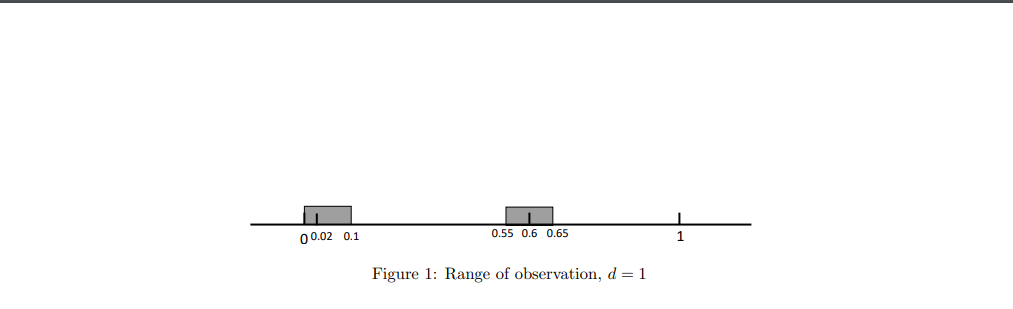
\includegraphics[width=0.8\textwidth]{section1.png}
        \caption{Primal Formulation of SVM}
        \label{fig:primal}
    \end{figure}
    \begin{itemize}
    \item  the range used for each feature is 10\% of the total range.
            \item Therefore, for each feature, the fraction of observations used is 0.1.
    
            \item Since \(X_1\) and \(X_2\) are independent, the joint probability is the product of the individual probabilities.
            \item Fraction used = \(0.1 \times 0.1 = 0.01\).
    \end{itemize}

    On average, we use 1\% of the available observations to make the prediction in two dimensions.
    
    
    \item On average, assuming $x_1$ and $x_2$ are each uniformly distributed on $[0, 1]$, what fraction of the available observations will we use to make the prediction?
    For a test observation \((x_1, x_2)\), we use training observations where:
\[
X_1 \in [x_1 - 0.05, x_1 + 0.05] \quad \text{and} \quad X_2 \in [x_2 - 0.05, x_2 + 0.05].
\]
If \(x_1\) or \(x_2\) is near the boundaries (\([0, 0.05)\) or \((0.95, 1]\)), the ranges are adjusted to stay within \([0, 1]\).


Since \(X_1\) and \(X_2\) are independent and uniformly distributed:
\begin{itemize}
    \item The fraction of observations used for \(X_1\) is \(0.1\) (10\% of the range).
    \item The fraction of observations used for \(X_2\) is \(0.1\) (10\% of the range).
\end{itemize}
The joint fraction of observations used is the product of the individual fractions:
\[
\text{Fraction used} = 0.1 \times 0.1 = 0.01.
\]


On average, we use \(1\%\) of the available observations to make the prediction in two dimensions.
    \item Now suppose that we have a set of training observations on $d = 100$ features. Again, the observations are uniformly distributed on each feature, and again each feature ranges in value from $0$ to $1$. We wish to predict a test observation’s response using observations within the $10\%$ of each feature’s range that is closest to that test observation. What fraction of the available observations will we use to make the prediction?
    \begin{itemize}
            \item The range used is 10\% of the total range, so the fraction for each feature is 0.1.
    
            \item Since all features are independent, the joint probability is the product of the individual probabilities.
            \item Fraction used = \(0.1^{100}\).
       
    \end{itemize}
    On average, we use \(0.1^{100}\) of the available observations to make the prediction in 100 dimensions.
    
    \item Using your answers to parts a–c, argue that a drawback of $k$-nearest neighbors when $d$ is large is that there are very few training observations “near” any given test observation.
    \\ The fraction of available observations used to make the prediction decreases exponentially with the number of dimensions. For example:
    \begin{itemize}
        \item In one dimension, we use 10\% of the observations.
        \item In two dimensions, we use 1\% of the observations.
        \item In 100 dimensions, we use \(0.1^{100}\) of the observations.
    \end{itemize}
    As the number of dimensions increases, the fraction of observations used to make the prediction decreases rapidly. This implies that there are very few training observations "near" any given test observation when the number of dimensions is large. As a result, the prediction may be based on very few observations, which can lead to high variance and poor generalization to new data.
    \item Now suppose that we wish to make a prediction for a test observation by creating a $d$-dimensional hypercube centered around the test observation that contains, on average, $10\%$ of the training observations. For $d = 1$, $2$, and $100$, what is the length of each side of the hypercube? How does your answer change as $d$ increases, and what does this imply for the accuracy of $k$-nearest neighbors when $d$ is large?
    
    \textbf{Note:} A hypercube is a generalization of a cube to an arbitrary number of dimensions. When $d = 1$, a hypercube is simply a line segment; when $d = 2$, it is a square; and when $d = 100$, it is a $100$-dimensional cube.
    
The volume of the hypercube is \(s^d = 0.1\), where \(s\) is the side length and \(d\) is the number of dimensions. Solving for \(s\):
\[
s = 0.1^{1/d}.
\]

\begin{itemize}
    \item \textbf{For \(d = 1\):} \(s = 0.1\).
    \item \textbf{For \(d = 2\):} \(s = \sqrt{0.1} \approx 0.316\).
    \item \textbf{For \(d = 100\):} \(s = 0.1^{1/100} \approx 0.977\).
\end{itemize}


As \(d\) increases, \(s\) grows and approaches 1. For example:
- At \(d = 1\), \(s = 0.1\).
- At \(d = 100\), \(s \approx 0.977\).


\begin{itemize}
    \item \textbf{Curse of Dimensionality:} In high dimensions, the hypercube must cover almost the entire feature space to capture 10\% of the data.
    \item \textbf{Sparsity of Data:} Data points become sparse, and distances between points grow, making "nearness" less meaningful.
    \item \textbf{Poor Performance:} k-NN struggles in high dimensions because it relies on finding meaningful neighbors, which becomes difficult due to data sparsity.
\end{itemize}


As \(d\) increases, the side length \(s\) approaches 1, illustrating the curse of dimensionality. This makes k-NN and other distance-based methods less effective in high-dimensional spaces.

\end{enumerate}
\newpage

\section{Decision Trees}
You obtained the following data from interviewing 15 people on the street. Based on a person’s relationship
status, age, education level and income, you can now build a decision tree to predict a person’s phone usage.
\begin{figure}[h]
    \centering
    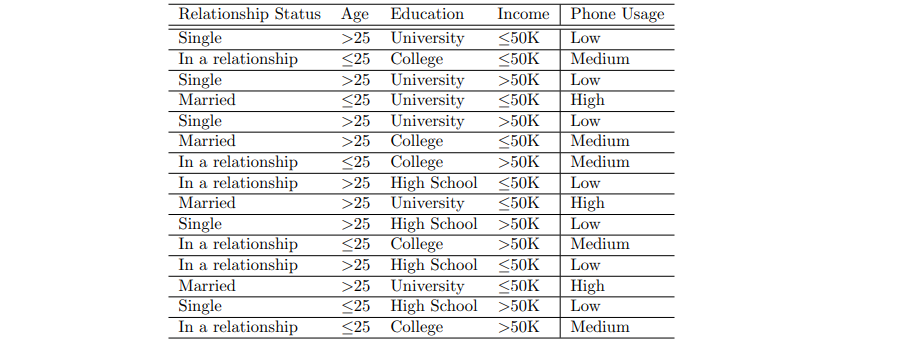
\includegraphics[width=0.8\textwidth]{section2.png}
    \caption{Primal Formulation of SVM}
    \label{fig:primal}
\end{figure}

\begin{enumerate}
    \item What is the entropy of Phone Usage? (Calculate entropy in log2 base and round to 4 decimal places)
    \[
    \text{Entropy} = -\sum_{i=1}^n p_i \log_2 p_i
    \]
    phone usage = \{low, medium, high\} = \{7, 5, 3\}
    \[
    \text{Entropy} = -\left(\frac{7}{15} \log_2 \frac{7}{15} + \frac{5}{15} \log_2 \frac{5}{15} + \frac{3}{15} \log_2 \frac{3}{15}\right)
    \]
    \[
    \text{Entropy} = -\left(0.4666 \times -1.0995356735715 + 0.3333 \times -1.5849625021639 + 0.2 \times -2.3219280948874\right)
    \]
    \[
    \text{Entropy} = -\left(-0.513043345 + -0.528268002 + -0.4643856189775\right)
    \]
    \[
    \text{Entropy} = -\left(-1.5056969659775\right)
    \]
    \[
    \text{Entropy} = \textbf{1.5056969659775}
    \]
    rounding to 4 decimal places:
    \[
    \text{Entropy} = \textbf{1.5057}
    \]
    \item Find the information gain (IG) from each feature (relationship status, age, education levarianceel and income). Which feature should be chosen at the root of the tree? Show your calculations for the information gain (IG) and explain your choice in a sentence. (Calculate entropy in log2 base and round to 4 decimal places)
    \\ \textbf{Information gain:}
    \[
    \text{IG}(\text{Feature}) = H(\text{Phone Usage}) - H(\text{Phone Usage} \mid \text{Feature}) = \text{ phone usage entropy} - \sum_{j=1}^m \frac{N_j}{N} \text{Entropy}(\text{Phone Usage} \mid \text{Feature} = j)
    \]
    where:
    \begin{itemize}
        \item $H(\text{Phone Usage})$ is the entropy of the phone usage.
        \item $H(\text{Phone Usage} \mid \text{Feature})$ is the conditional entropy of the phone usage given the feature.
        \item $N_j$ is the number of samples in the dataset with the feature value $j$.
        \item $N$ is the total number of samples in the dataset.
        \item $m$ is the number of unique values of the feature.
        \item $\text{Entropy}(\text{Phone Usage} \mid \text{Feature} = j)$ is the entropy of the phone usage given the feature value $j$.
    \end{itemize}
    \textbf{relationship status}
    \[
    \text{Entropy} = -\sum_{i=1}^n p_i \log_2 p_i
    \]
    relationship status = \{single, married, in a relationship\} = \{5, 4, 6\}
    \\ single = \{low, medium, high\} = \{5, 0, 0\}
    \\ married = \{low, medium, high\} = \{0, 1, 3\}
    \\ in a relationship = \{low, medium, high\} = \{2, 4, 0\}
    \\ \textbf{entropy of phone usage given relationship status:}
    \[
    \text{Entropy (Phone Usage} \mid \text{relationship status)} = \sum_{j=1}^m \frac{N_j}{N} \text{Entropy}(\text{Phone Usage} \mid \text{relationship status} = j)
    \]
    Entropy (Phone Usage $\mid$ single):
    \[
    \text{Entropy} = -\left(\frac{5}{5} \log_2 \frac{5}{5} + \frac{0}{5} \log_2 \frac{0}{5} + \frac{0}{5} \log_2 \frac{0}{5}\right)
    \]
    \[
    \text{Entropy} = -\left(1 \times 0 + 0 \times -\infty + 0 \times -\infty\right)
    \]
    \[
    \text{Entropy} = -\left(0\right)
    \]
    \[
    \text{Entropy} = \textbf{0}
    \]
    Entropy (Phone Usage $\mid$ in a relationship):
    \[
    \text{Entropy} = -\left(\frac{2}{6} \log_2 \frac{2}{6} + \frac{4}{6} \log_2 \frac{4}{6} + \frac{0}{6} \log_2 \frac{0}{6}\right)
    \]
    \[
    \text{Entropy} = -\left(0.3333 \times -1.5849625021639 + 0.6666 \times -0.5849625 + 0 \times -\infty\right)
    \]
    \[
    \text{Entropy} = -\left(-0.528268002 - 0.389936002 + 0\right)
    \]
    \[
    \text{Entropy} = -\left(-0.918204004\right)
    \]
    \[
    \text{Entropy} = \textbf{0.918204004}
    \]
    Entropy (Phone Usage $\mid$ married):
    \[
    \text{Entropy} = -\left(\frac{0}{4} \log_2 \frac{0}{4} + \frac{1}{4} \log_2 \frac{1}{4} + \frac{3}{4} \log_2 \frac{3}{4}\right)
    \]
    \[
    \text{Entropy} = -\left(0 \times -\infty + 0.25 \times -2 + 0.75 \times -0.41503749927884\right)
    \]
    \[
    \text{Entropy} = -\left(0 + -0.5 + -0.31127762445913\right)
    \]
    \[
    \text{Entropy} = -\left(-0.81127762445913\right)
    \]
    \[
    \text{Entropy} = \textbf{0.81127762445913}
    \]
    Entropy (Phone Usage $\mid$ relationship status):
    \[
    \text{Entropy (Phone Usage} \mid \text{relationship status)} = \sum_{j=1}^m \frac{N_j}{N} \text{Entropy}(\text{Phone Usage} \mid \text{relationship status} = j)
    \]
    \[
    \text{Entropy (Phone Usage} \mid \text{relationship status)} = \frac{5}{15} \times 0 + \frac{6}{15} \times 0.918204004 + \frac{4}{15} \times 0.81127762445913
    \]
    \[
    \text{Entropy (Phone Usage} \mid \text{relationship status)} = 0 + 0.367282402 + 0.216340699
    \]
    \[
    \text{Entropy (Phone Usage} \mid \text{relationship status)} = 0.583623101
    \]
    information gain:
    \[
    \text{IG}(\text{relationship status}) = 1.5057 - 0.583623101
    \]
    \[
    \text{IG}(\text{relationship status}) = \textbf{0.922076898}
    \]
    \textbf{age}
    \[
    \text{Entropy} = -\sum_{i=1}^n p_i \log_2 p_i
    \]
    age = $\{>25, \leq 25\} = \{9, 6\}$
    \\ $>25$ = \{low, medium, high\} = \{6, 1, 2\}
    \\ $ \leq 25 = \{low, \text{medium}, \text{high}\} = \{1, 4, 1\} $
    \\ \textbf{entropy of phone usage given age:}
    \[
    \text{Entropy (Phone Usage} \mid \text{age)} = \sum_{j=1}^m \frac{N_j}{N} \text{Entropy}(\text{Phone Usage} \mid \text{age} = j)
    \]
    Entropy (Phone Usage $\mid$ $>25$):
    \[
    \text{Entropy} = -\left(\frac{6}{9} \log_2 \frac{6}{9} + \frac{1}{9} \log_2 \frac{1}{9} + \frac{2}{9} \log_2 \frac{2}{9}\right)
    \]
    \[
    \text{Entropy} = -\left(0.6666 \times -0.5849625 + 0.1111 \times -3.1699250014423 + 0.2222 \times -2.1699250014423\right)
    \]
    \[
    \text{Entropy} = -\left(-0.389936002 - 0.352182778 - 0.481983334\right)
    \]
    \[
    \text{Entropy} = -\left(- 1.224319514\right)
    \]
    \[
    \text{Entropy} = \textbf{1.224319514}
    \]
    Entropy (Phone Usage $\mid$ $\leq 25$):
    \[
    \text{Entropy} = -\left(\frac{1}{6} \log_2 \frac{1}{6} + \frac{4}{6} \log_2 \frac{4}{6} + \frac{1}{6} \log_2 \frac{1}{6}\right)
    \]
    \[
    \text{Entropy} = -\left(0.1666 \times -2.5849625007212 + 0.6666 \times -0.5849625 + 0.1666 \times -2.5849625007212\right)
    \]
    \[
    \text{Entropy} = -\left(-0.430827083 - 0.389936002 - 0.430827083\right)
    \]
    \[
    \text{Entropy} = -\left(- 1.251590168\right)
    \]
    \[
    \text{Entropy} = \textbf{1.251590168}
    \]
    Entropy (Phone Usage $\mid$ age):
    \[
    \text{Entropy (Phone Usage} \mid \text{age)} = \sum_{j=1}^m \frac{N_j}{N} \text{Entropy}(\text{Phone Usage} \mid \text{age} = j)
    \]
    \[
    \text{Entropy (Phone Usage} \mid \text{age)} = \frac{9}{15} \times 1.224319514 + \frac{6}{15} \times 1.251590168
    \]
    \[
    \text{Entropy (Phone Usage} \mid \text{age)} = 0.734591708 + 0.500793445
    \]
    \[
    \text{Entropy (Phone Usage} \mid \text{age)} = 1.235385153
    \]
    information gain:
    \[
    \text{IG}(\text{age}) = 1.5057 - 1.235385153
    \]
    \[
    \text{IG}(\text{age}) = \textbf{0.270314847}
    \]
    \textbf{education level}
    \[
    \text{Entropy} = -\sum_{i=1}^n p_i \log_2 p_i
    \]
    education level = \{high school, college, University\} = \{4, 5, 6\}
    \\ high school = \{low, medium, high\} = \{4, 0, 0\}
    \\ college = \{low, medium, high\} = \{0, 5, 0\}
    \\ university = \{low, medium, high\} = \{3, 0, 3\}
    \\ \textbf{entropy of phone usage given education level:}
    \[
    \text{Entropy (Phone Usage} \mid \text{education level)} = \sum_{j=1}^m \frac{N_j}{N} \text{Entropy}(\text{Phone Usage} \mid \text{education level} = j)
    \]
    Entropy (Phone Usage $\mid$ high school):
    \[
    \text{Entropy} = -\left(\frac{4}{4} \log_2 \frac{4}{4} + \frac{0}{4} \log_2 \frac{0}{4} + \frac{0}{4} \log_2 \frac{0}{4}\right)
    \]
    \[
    \text{Entropy} = -\left(1 \times 0 + 0 \times -\infty + 0 \times -\infty\right)
    \]
    \[
    \text{Entropy} = -\left(0\right)
    \]
    \[
    \text{Entropy} = \textbf{0}
    \]
    Entropy (Phone Usage $\mid$ university):
    \[
    \text{Entropy} = -\left(\frac{3}{6} \log_2 \frac{3}{6} + \frac{0}{6} \log_2 \frac{0}{6} + \frac{3}{6} \log_2 \frac{3}{6}\right)
    \]
    \[
    \text{Entropy} = -\left(0.5 \times -1 + 0 \times -\infty + 0.5 \times -1\right)
    \]
    \[
    \text{Entropy} = -\left(-0.5 + 0 + -0.5\right)
    \]
    \[
    \text{Entropy} = -\left(-1\right)
    \]
    \[
    \text{Entropy} = \textbf{1}
    \]
    Entropy (Phone Usage $\mid$ college):
    \[
    \text{Entropy} = -\left(\frac{0}{5} \log_2 \frac{0}{5} + \frac{5}{5} \log_2 \frac{5}{5} + \frac{0}{5} \log_2 \frac{0}{5}\right)
    \]
    \[
    \text{Entropy} = -\left(0 \times -\infty + 1 \times 0 + 0 \times -\infty\right)
    \]
    \[
    \text{Entropy} = -\left(0 + 0 + 0\right)
    \]
    \[
    \text{Entropy} = \textbf{0}
    \]
    Entropy (Phone Usage $\mid$ education level):
    \[
    \text{Entropy (Phone Usage} \mid \text{education level)} = \sum_{j=1}^m \frac{N_j}{N} \text{Entropy}(\text{Phone Usage} \mid \text{education level} = j)
    \]
    \[
    \text{Entropy (Phone Usage} \mid \text{education level)} = \frac{4}{15} \times 0 + \frac{6}{15} \times 1 + \frac{5}{15} \times 0
    \]
    \[
    \text{Entropy (Phone Usage} \mid \text{education level)} = 0 + 0.4 + 0
    \]
    \[
    \text{Entropy (Phone Usage} \mid \text{education level)} = 0.4
    \]
    information gain:
    \[
    \text{IG}(\text{education level}) = 1.5057 - 0.4
    \]
    \[
    \text{IG}(\text{education level}) = \textbf{1.1057}
    \]
    \textbf{income}
    \[
    \text{Entropy} = -\sum_{i=1}^n p_i \log_2 p_i
    \]
    income = $\{\leq 50K, > 50K\}$ = $\{8, 7\}$
    \\ $\leq 50K$ = \{low, medium, high\} = \{3, 2, 3\}
    \\ $> 50K$ = \{low, medium, high\} = \{4, 3, 0\}
    \\ \textbf{entropy of phone usage given income:}
    \[
    \text{Entropy (Phone Usage} \mid \text{income)} = \sum_{j=1}^m \frac{N_j}{N} \text{Entropy}(\text{Phone Usage} \mid \text{income} = j)
    \]
    Entropy (Phone Usage $\mid$ $\leq 50K$):
    \[
    \text{Entropy} = -\left(\frac{3}{8} \log_2 \frac{3}{8} + \frac{2}{8} \log_2 \frac{2}{8} + \frac{3}{8} \log_2 \frac{3}{8}\right)
    \]
    \[
    \text{Entropy} = -\left(0.375 \times -1.415037499 + 0.25 \times -2 + 0.375 \times -1.415037499\right)
    \]
    \[
    \text{Entropy} = -\left(-0.530639062 + -0.5 + -0.530639062\right)
    \]
    \[
    \text{Entropy} = -\left(-1.561278124\right)
    \]
    \[
    \text{Entropy} = \textbf{1.561278124}
    \]
    Entropy (Phone Usage $\mid$ $> 50K$):
    \[
    \text{Entropy} = -\left(\frac{4}{7} \log_2 \frac{4}{7} + \frac{3}{7} \log_2 \frac{3}{7} + \frac{0}{7} \log_2 \frac{0}{7}\right)
    \]
    \[
    \text{Entropy} = -\left(0.5714 \times -0.807354922 + 0.4286 \times -1.222392421 + 0 \times -\infty\right)
    \]
    \[
    \text{Entropy} = -\left(-0.461345669 - 0.523917391 + 0\right)
    \]
    \[
    \text{Entropy} = -\left(-0.985239993\right)
    \]
    \[
    \text{Entropy} = \textbf{0.985239993}
    \]
    Entropy (Phone Usage $\mid$ income):
    \[
    \text{Entropy (Phone Usage} \mid \text{income)} = \sum_{j=1}^m \frac{N_j}{N} \text{Entropy}(\text{Phone Usage} \mid \text{income} = j)
    \]
    \[
    \text{Entropy (Phone Usage} \mid \text{income)} = \frac{8}{15} \times 1.561278124 + \frac{7}{15} \times 0.985239993
    \]
    \[
    \text{Entropy (Phone Usage} \mid \text{income)} = 0.832681666 + 0.459131995
    \]
    \[
    \text{Entropy (Phone Usage} \mid \text{income)} = 1.291813661
    \]
    information gain:
    \[
    \text{IG}(\text{income}) = 1.5057 - 1.291813661
    \]
    \[
    \text{IG}(\text{income}) = \textbf{0.213886339}
    \]
    Final information gains:
    \[
    \text{IG}(\text{relationship status}) = \textbf{0.9221}
    \]
    \[
    \text{IG}(\text{age}) = \textbf{0.27031}
    \]
    \[
    \text{IG}(\text{education level}) = \textbf{1.1057}
    \]
    \[
    \text{IG}(\text{income}) = \textbf{0.2139 }
    \]
    The feature with the highest information gain is the \textbf{education level}. Therefore, the education level should be chosen at the root of the tree.



    \item  Use the root you found in part (b) to determine the rest of the nodes in the decision tree for the abovariancee data. Draw the full decision tree, i.e., keep splitting the nodes until further splits do not lead to any information gain (you may not need all the features for this). For each split, show your working on why you chose this feature based on information gain.
    \begin{center}
        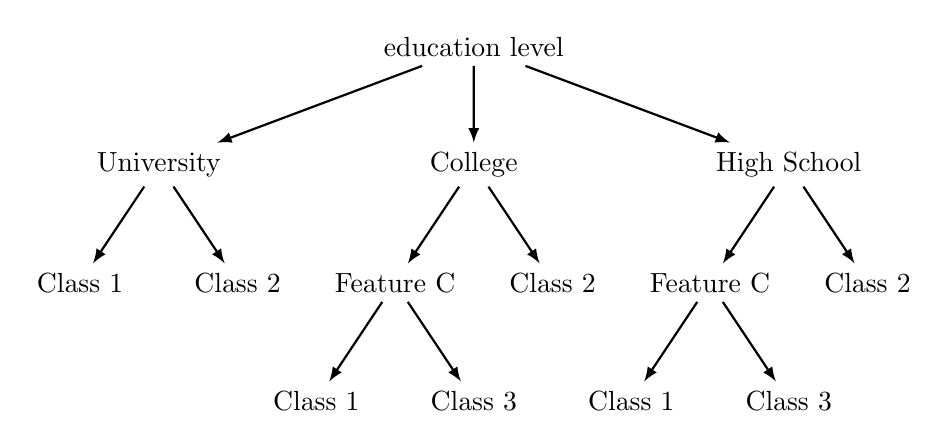
\begin{tikzpicture}[
          level distance=1.5cm,
          level 1/.style={sibling distance=4cm},
          level 2/.style={sibling distance=2cm},
          edge from parent/.style={draw, thick, -latex}
        ]
        
        \node {education level}
            child { node {University } 
                child { node {Class 1} }
                child { node {Class 2} }
            }
            child { node {College}
                child { node {Feature C} 
                    child { node {Class 1} }
                    child { node {Class 3} }
                }
                child { node {Class 2} }
            }
            child { node {High School}
                child { node {Feature C} 
                    child { node {Class 1} }
                    child { node {Class 3} }
                }
                child { node {Class 2} }
            };
        
        \end{tikzpicture}
        \end{center}
\end{enumerate}
\newpage
\section{Random Forests}
Consider the data samples in Table 1, which record whether a person gets sick, together with features about their age ($A$), social distancing ($S$), and hand-washing frequency ($H$). Our goal is to learn a random forest to predict whether the person is prone to getting sick.
\begin{table}[h!]
    \centering
    \begin{tabular}{|c|c|c|c|c|}
    \hline
    \textbf{Sample} & \textbf{Age (A)} & \textbf{Social Distancing (S)} & \textbf{Hand Washing (H)} & \textbf{Getting Sick} \\ \hline
    1 & Old & Yes & Yes & No \\ \hline
    2 & Old & Yes & No & No \\ \hline
    3 & Old & Yes & Yes & No \\ \hline
    4 & Young & No & No & Yes \\ \hline
    5 & Young & Yes & Yes & No \\ \hline
    6 & Old & No & No & Yes \\ \hline
    7 & Old & No & Yes & Yes \\ \hline
    8 & Old & No & No & Yes \\ \hline
    \end{tabular}
    \caption{}
    \label{table:data}
    \end{table}

    Instead of using all features to build a single decision tree, we decide to use the random forest algorithm. Specifically, we will build three trees, each using only two features, and then combine their outcomes for the final prediction.

    \begin{enumerate}
        \item  Build 3 decision trees using two features out of the three for each tree. Use information gain to decide the feature to split on. Use majority voting if all the samples in a leaf node do not have the same label.
        \\ Entropy of Getting Sick:
        \[
        \text{Entropy} = -\sum_{i=1}^n p_i \log_2 p_i
        \]
        getting sick = \{yes, no\} = \{4, 4\}
        \[
        \text{Entropy} = -\left(\frac{4}{8} \log_2 \frac{4}{8} + \frac{4}{8} \log_2 \frac{4}{8}\right)
        \]
        \[
        \text{Entropy} = -\left(0.5 \times -1 + 0.5 \times -1\right)
        \]
        \[
        \text{Entropy} = -\left(-0.5 + -0.5\right)
        \]
        \[
        \text{Entropy} = -\left(-1\right)
        \]
        \[
        \text{Entropy} = \textbf{1}
        \]
        Entropy of Getting Sick given Age:
        \[
        \text{Entropy (Getting Sick} \mid \text{Age)} = \sum_{j=1}^m \frac{N_j}{N} \text{Entropy}(\text{Getting Sick} \mid \text{Age} = j)
        \]
        Age = \{old, young\} = \{6, 2\}
        \\ old = \{yes, no\} = \{3, 3\}
        \\ young = \{yes, no\} = \{1, 1\}
        \\ \textbf{entropy of getting sick given age:}
        \[
        \text{Entropy (Getting Sick} \mid \text{Age)} = \sum_{j=1}^m \frac{N_j}{N} \text{Entropy}(\text{Getting Sick} \mid \text{Age} = j)
        \]
        Entropy (Getting Sick $\mid$ old):
        \[
        \text{Entropy} = -\left(\frac{3}{6} \log_2 \frac{3}{6} + \frac{3}{6} \log_2 \frac{3}{6}\right)
        \]
        \[
        \text{Entropy} = -\left(0.5 \times -1 + 0.5 \times -1\right)
        \]
        \[
        \text{Entropy} = -\left(-0.5 + -0.5\right)
        \]
        \[
        \text{Entropy} = -\left(-1\right)
        \]
        \[
        \text{Entropy} = \textbf{1}
        \]
        Entropy (Getting Sick $\mid$ young):
        \[
        \text{Entropy} = -\left(\frac{1}{2} \log_2 \frac{1}{2} + \frac{1}{2} \log_2 \frac{1}{2}\right)
        \]
        \[
        \text{Entropy} = -\left(0.5 \times -1 + 0.5 \times -1\right)
        \]
        \[
        \text{Entropy} = -\left(-0.5 + -0.5\right)
        \]
        \[
        \text{Entropy} = -\left(-1\right)
        \]
        \[
        \text{Entropy} = \textbf{1}
        \]
        \[
        \text{Entropy (Getting Sick} \mid \text{Age)} = \frac{6}{8} \times 1 + \frac{2}{8} \times 1
        \]
        \[
        \text{Entropy (Getting Sick} \mid \text{Age)} = 0.75 + 0.25
        \]
        \[
        \text{Entropy (Getting Sick} \mid \text{Age)} = 1
        \]
        information gain:
        \[
        \text{IG}(\text{Age}) = 1 - 1
        \]
        \[
        \text{IG}(\text{Age}) = \textbf{0}
        \]
        Entropy of Getting Sick given Social Distancing:
        \[
        \text{Entropy (Getting Sick} \mid \text{Social Distancing)} = \sum_{j=1}^m \frac{N_j}{N} \text{Entropy}(\text{Getting Sick} \mid \text{Social Distancing} = j)
        \]
        Social Distancing = \{yes, no\} = \{4, 4\}
        \\ yes = \{yes, no\} = \{0, 4\}
        \\ no = \{yes, no\} = \{4, 0\}
        \\ \textbf{entropy of getting sick given social distancing:}
        \[
        \text{Entropy (Getting Sick} \mid \text{Social Distancing)} = \sum_{j=1}^m \frac{N_j}{N} \text{Entropy}(\text{Getting Sick} \mid \text{Social Distancing} = j)
        \]
        Entropy (Getting Sick $\mid$ yes):
        \[
        \text{Entropy} = -\left(\frac{0}{4} \log_2 \frac{0}{4} + \frac{4}{4} \log_2 \frac{4}{4}\right)
        \]
        \[
        \text{Entropy} = -\left(0 \times -\infty + 1 \times 0\right)
        \]
        \[
        \text{Entropy} = -\left(0 + 0\right)
        \]
        \[
        \text{Entropy} = \textbf{0}
        \]
        Entropy (Getting Sick $\mid$ no):
        \[
        \text{Entropy} = -\left(\frac{4}{4} \log_2 \frac{4}{4} + \frac{0}{4} \log_2 \frac{0}{4}\right)
        \]
        \[
        \text{Entropy} = -\left(1 \times 0 + 0 \times -\infty\right)
        \]
        \[
        \text{Entropy} = -\left(0 + 0\right)
        \]
        \[
        \text{Entropy} = \textbf{0}
        \]
        \[
        \text{Entropy (Getting Sick} \mid \text{Social Distancing)} = \frac{4}{8} \times 0 + \frac{4}{8} \times 0
        \]
        \[
        \text{Entropy (Getting Sick} \mid \text{Social Distancing)} = 0 + 0
        \]
        \[
        \text{Entropy (Getting Sick} \mid \text{Social Distancing)} = \textbf{0}
        \]
        information gain:
        \[
        \text{IG}(\text{Social Distancing}) = 1 - 0
        \]
        \[
        \text{IG}(\text{Social Distancing}) = \textbf{1}
        \]
        Entropy of Getting Sick given Hand Washing:
        \[
        \text{Entropy (Getting Sick} \mid \text{Hand Washing)} = \sum_{j=1}^m \frac{N_j}{N} \text{Entropy}(\text{Getting Sick} \mid \text{Hand Washing} = j)
        \]
        Hand Washing = \{yes, no\} = \{4, 4\}
        \\ yes = \{yes, no\} = \{3, 1\}
        \\ no = \{yes, no\} = \{1, 3\}
        \\ \textbf{entropy of getting sick given hand washing:}
        \[
        \text{Entropy (Getting Sick} \mid \text{Hand Washing)} = \sum_{j=1}^m \frac{N_j}{N} \text{Entropy}(\text{Getting Sick} \mid \text{Hand Washing} = j)
        \]
        Entropy (Getting Sick $\mid$ yes):
        \[
        \text{Entropy} = -\left(\frac{3}{4} \log_2 \frac{3}{4} + \frac{1}{4} \log_2 \frac{1}{4}\right)
        \]
        \[
        \text{Entropy} = -\left(0.75 \times -0.41503749927884 + 0.25 \times -2\right)
        \]
        \[
        \text{Entropy} = -\left(-0.31127762445913 - 0.5\right)
        \]
        \[
        \text{Entropy} = -\left(-0.81127762445913\right)
        \]
        \[
        \text{Entropy} = \textbf{0.81127762445913}
        \]
        Entropy (Getting Sick $\mid$ no):
        \[
        \text{Entropy} = -\left(\frac{1}{4} \log_2 \frac{1}{4} + \frac{3}{4} \log_2 \frac{3}{4}\right)
        \]
        \[
        \text{Entropy} = -\left(0.25 \times -2 + 0.75 \times -0.41503749927884\right)
        \]
        \[
        \text{Entropy} = -\left(-0.5 + -0.31127762445913\right)
        \]
        \[
        \text{Entropy} = -\left(-0.81127762445913\right)
        \]
        \[
        \text{Entropy} = \textbf{0.81127762445913}
        \]
        \[
        \text{Entropy (Getting Sick} \mid \text{Hand Washing)} = \frac{4}{8} \times 0.81127762445913 + \frac{4}{8} \times 0.81127762445913
        \]
        \[
        \text{Entropy (Getting Sick} \mid \text{Hand Washing)} = 0.40563881222957 + 0.40563881222957
        \]
        \[
        \text{Entropy (Getting Sick} \mid \text{Hand Washing)} = 0.81127762445913
        \]
        information gain:
        \[
        \text{IG}(\text{Hand Washing}) = 1 - 0.81127762445913
        \]
        \[
        \text{IG}(\text{Hand Washing}) = \textbf{0.18872237554087}
        \]
        Tree 1: Age and Social Distancing, social distance is chosen as the root node.\\
        \begin{tikzpicture}[
            level distance=1.5cm,
            level 1/.style={sibling distance=10cm},
            level 2/.style={sibling distance=7cm},
            level 3/.style={sibling distance=5cm},
            edge from parent/.style={draw, thick, -latex}
        ]

        \node {Social Distancing}
                child { node {Yes}
                        child { node {Age}
                                child { node {Old}
                                        child { node {Getting sick}
                                        child { node {No (3)} }
                                }
                                }
                                child { node {Young}
                                        child { node {Getting sick}
                                        child { node {Yes (1)} }
                                }
                                }
                            }
                }
                child { node {No}
                        child { node {Age}
                                child { node {Old}
                                        child { node {Getting sick}
                                        child { node {Yes (3)} }
                                }
                                }
                                child { node {Young}
                                        child { node {Getting sick}
                                        child { node {No (1)} }
                                }
                                }
                        }
                };

        \end{tikzpicture}
        \\ For the second tree, we will use the features age and hand washing.hand washing is chosen as the root node.\\
        \begin{tikzpicture}[
            level distance=1.5cm,
            level 1/.style={sibling distance=10cm},
            level 2/.style={sibling distance=7cm},
            level 3/.style={sibling distance=5cm},
            edge from parent/.style={draw, thick, -latex}
        ]
        \node {Hand Washing}
            child { node {Yes}
            child { node {Age}
                child { node {Old}
                child { node {Getting sick}
                    child { node {Yes (1)} }
                    child { node {No (2)} }
                }
                }
                child { node {Young}
                child { node {Getting sick}
                    child { node {No (1)} }
                }
                }
            }
            }
            child { node {No}
            child { node {Age}
                child { node {Old}
                child { node {Getting sick}
                    child { node {Yes (2)} }
                    child { node {No (1)} }
                }
                }
                child { node {Young}
                child { node {Getting sick}
                    child { node {No (1)} }
                }
                }
            }
            };
        \end{tikzpicture}
        \\ For the third tree, we will use the features social distancing and hand washing. social distancing is chosen as the root node.\\
        \begin{tikzpicture}[
            level distance=1.5cm,
            level 1/.style={sibling distance=10cm},
            level 2/.style={sibling distance=7cm},
            level 3/.style={sibling distance=5cm},
            edge from parent/.style={draw, thick, -latex}
        ]
        \node {Social Distancing}
            child { node {Yes}
            child { node {Hand Washing}
                child { node {Yes}
                child { node {Getting sick}
                    child { node {No (3)} }
                }
                }
                child { node {No}
                child { node {Getting sick}
                    child { node {No (1)} }
                }
                }
            }
            }
            child { node {No}
            child { node {Hand Washing}
                child { node {Yes}
                child { node {Getting sick}
                    child { node {Yes (1)} }
                }
                }
                child { node {No}
                child { node {Getting sick}
                    child { node {Yes (3)} }
                }
                }
            }
            };
        \end{tikzpicture}
        
        \item  Given a new data point with the features ($A = \text{old}$, $S = \text{yes}$, $H = \text{no}$), use the trees you learned from part (a) to predict whether this person will get sick.
        \\ For the first tree, the person will get sick.
        \\ For the second tree, the person will get sick.
        \\ For the third tree, the person will not get sick.
        The person will get sick according to two trees and will not get sick according to one tree. Therefore, the final prediction is that the person will get sick.
        \item  Briefly (in 1-2 sentences) comment on the advantage of random forests over decision trees from the perspective of bias-variance trade-off.
        \\ Random forests reduce the variance of the model by training multiple decision trees on different subsets of the data and features. This ensemble method helps to reduce overfitting and improve the generalization of the model.
    \end{enumerate}

\newpage
\section{Adaboost}
Recall the AdaBoost algorithm for classification of a training dataset $(x_n, y_n)$ for $n = 1, \dots, N$ and $y \in \{-1, 1\}$. AdaBoost sequentially combines $T$ weak classifiers $h_1(x), h_2(x), \dots, h_T(x)$ to build one strong classifier $\text{sign}(f_T(x))$. The steps of the algorithm are as follows:

\begin{itemize}
    \item \textbf{Initialize the weights:} $w_1(n) = \frac{1}{N}$, for all points $n = 1, 2, \dots, N$.
    \item \textbf{For $t = 1, \dots, T$:}
    \begin{itemize}
        \item \textbf{a.} Learn classifier $h_t(x)$ that minimizes the error:
        \[
        \epsilon_t = \sum_{n=1}^N w_t(n) \cdot \mathbb{1}(y_n \neq h_t(x_n)).
        \]
        \item \textbf{b.} Update the contribution:
        \[
        \beta_t = \frac{1}{2} \log_2\left(\frac{1 - \epsilon_t}{\epsilon_t}\right).
        \]
        \item \textbf{c.} Update weights of training points:
        \[
        w_{t+1}(n) \propto w_t(n) \cdot 2^{-\beta_t y_n h_t(x_n)},
        \]
        where the weights are normalized to ensure that $\sum_{n=1}^N w_{t+1}(n) = 1$.
    \end{itemize}
    \item \textbf{Return the final classifier:} $\text{sign}(f_T(x))$, where
    \[
    f_T(x) = \sum_{t=1}^T \beta_t h_t(x) \quad \text{for a given } x.
    \]
\end{itemize}

\textbf{Note:} The difference from the algorithm described during the lecture is that we have replaced $\log_e$ by $\log_2$ and $e^{-\beta_t}$ by $2^{-\beta_t}$ everywhere.
\begin{figure}[h]
    \centering
    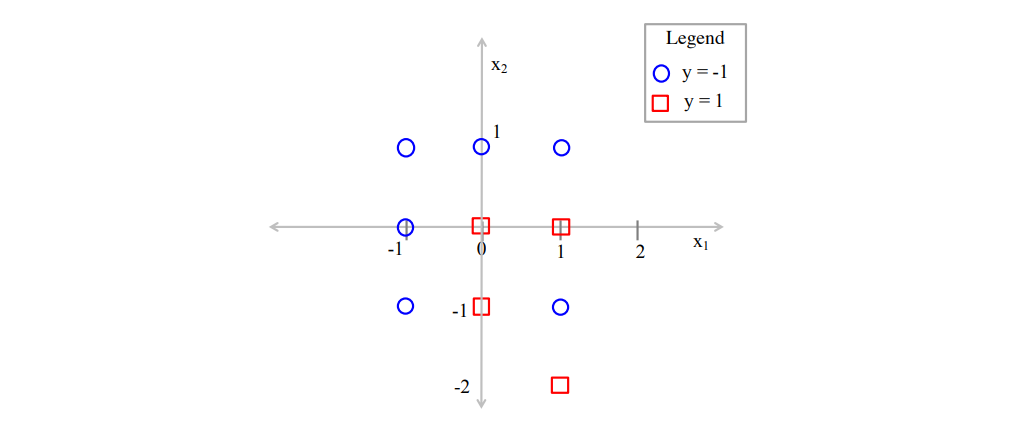
\includegraphics[width=0.8\textwidth]{adaboost.png}
    \caption{Primal Formulation of SVM}
    \label{fig:primal}
\end{figure}

Consider the training dataset with $N = 10$ points and two-dimensional features $x = (x_1, x_2)$ as shown in the figure above. In this problem, we will use a binary linear decision boundary as the base classifier and perform two iterations of AdaBoost.

\begin{enumerate}
    \item  Starting with equal weights $w_1(n) = \frac{1}{10}$ for all $N = 10$ points, which of the decision boundaries shown below gives the lowest error $\epsilon_1$? Select one of the following answers:

\begin{enumerate}
    \item Predict $y = 1$ if $x_2 \leq 0.5$.
    \item  Predict $y = 1$ if $-x_1 + x_2 \leq -0.5$.
    \item  Predict $y = 1$ if $-x_1 + x_2 \leq 0.5$.
\end{enumerate}

\begin{figure}[h!]
    \centering
    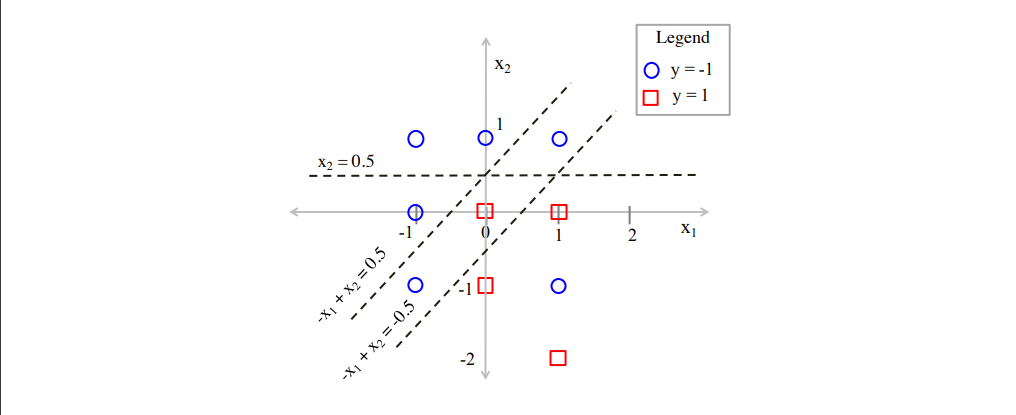
\includegraphics[width=0.8\textwidth]{adaboost2.png}
    \caption{Primal Formulation of SVM}
    \label{fig:primal}
\end{figure}


    \item Compute the error $\epsilon_1$ and the contribution $\beta_1$ of the decision boundary that you chose in part (a) above.

\item  Compute the updated and normalized weights $w_2(n)$ of each of the data points as follows:

\begin{table}[h!]
\centering
\begin{tabular}{|c|c|c|}
\hline
\textbf{n} & \textbf{Coordinates} & \textbf{$w_2(n)$} \\ \hline
1. & $(-1, 1)$ & \\ \hline
2. & $(0, 1)$ & \\ \hline
3. & $(1, 1)$ & \\ \hline
4. & $(-1, 0)$ & \\ \hline
5. & $(0, 0)$ & \\ \hline
6. & $(1, 0)$ & \\ \hline
7. & $(-1, -1)$ & \\ \hline
8. & $(0, -1)$ & \\ \hline
9. & $(1, -1)$ & \\ \hline
10. & $(1, -2)$ & \\ \hline
\end{tabular}
\caption{}
\label{table:weights}
\end{table}

\item Suppose you are given one more weak classifier that predicts $y = 1$ if $1.5x_1 + x_2 \leq 0.5$, as shown in the figure below. Compute the contribution $\beta_2$ of this classifier for the updated set of weights $w_2(n)$. Use the approximation $\log_2 3 \approx 1.6$.

\item Combine the new classifier with the classifier that you obtained in part (a). Specify the label $y \in \{-1, 1\}$ predicted by this combined classifier for each data point. Do you observe any change in the prediction, compared to the prediction from only using part (a)'s classifier?

\item  If we continue adding more classifiers, each with error less than $0.5$, how does the training error of the combined classifier $f_T(x)$ change? Briefly explain your answer in 1-2 sentences.

\newpage
\section{Neural Networks}
Below is a deep network with inputs $x_1, x_2$. The internal nodes and activation functions are as shown in the figure and equations below. All variables are scalar values, and $\exp(x)$ refers to the function $e^x$. The activation functions of the nodes $h_1, h_2, h_3$ are ReLU (i.e., $r_1 = \max(h_1, 0)$ etc.), for node $s_1$ we have $s_1 = \max(r_2, r_3)$, and for the other nodes:
\[
y_1 = \frac{\exp(r_1)}{\exp(r_1) + \exp(s_1)}, \quad y_2 = \frac{\exp(s_1)}{\exp(r_1) + \exp(s_1)}, \quad z = y_1 + y_2.
\]
\begin{figure}[h]
    \centering
    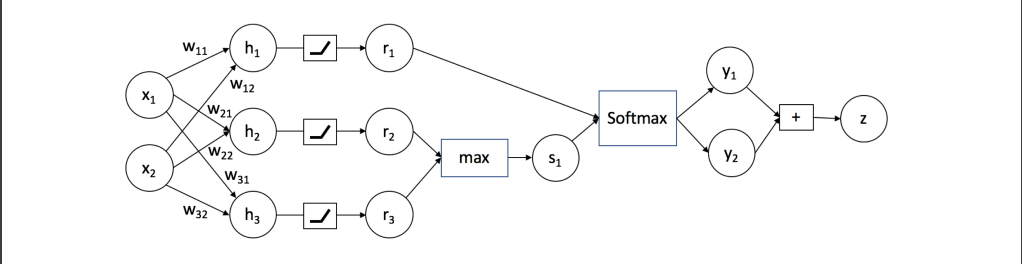
\includegraphics[width=0.8\textwidth]{Neural.png}
    \caption{Primal Formulation of SVM}
    \label{fig:primal}
\end{figure}
\begin{enumerate}
    \item \textbf{Forward propagation}Now,  Given $x_1 = 1$, $x_2 = -2$, $w_{11} = 6$, $w_{12} = 2$, $w_{21} = 4$, $w_{22} = 7$, $w_{31} = 5$, $w_{32} = 1$, compute the values of the internal nodes (shown in the table below). You may leave $e$ in your answer.

\begin{table}[h!]
\centering
\begin{tabular}{|c|c|c|c|c|c|c|c|c|c|}
\hline
$h_1$ & $h_2$ & $h_3$ & $r_1$ & $r_2$ & $r_3$ & $s_1$ & $y_1$ & $y_2$ & $z$ \\ \hline
 & & & & & & & & & \\ \hline
\end{tabular}
\caption{Values of internal nodes after forward propagation.}
\label{table:forward}
\end{table}

\item \textbf{Bounds on Variables}
\begin{itemize}
    \item Find the range of feasible values for $y_1$.
    \item Find the range of feasible values for $z$.
\end{itemize}

\item \textbf{Backpropagation}
Compute the gradient expressions shown in the table below analytically. The answer should be an expression that may include any of the nodes in the network ($x_1, x_2, h_1, h_2, h_3, r_1, r_2, r_3, s_1, y_1, y_2, z$) or weights ($w_{11}, w_{12}, w_{21}, w_{22}, w_{31}, w_{32}$).

\begin{table}[h!]
\centering
\begin{tabular}{|c|c|}
\hline
\textbf{Gradient} & \textbf{Expression} \\ \hline
$\frac{\partial h_1}{\partial w_{12}}$ & \\ \hline
$\frac{\partial h_1}{\partial x_1}$ & \\ \hline
$\frac{\partial r_1}{\partial h_1}$ & \\ \hline
$\frac{\partial y_1}{\partial r_1}$ & \\ \hline
$\frac{\partial y_1}{\partial s_1}$ & \\ \hline
$\frac{\partial z}{\partial y_1}$ & \\ \hline
$\frac{\partial z}{\partial x_1}$ & \\ \hline
$\frac{\partial s_1}{\partial r_2}$ & \\ \hline
\end{tabular}
\caption{Gradient expressions for backpropagation.}
\label{table:gradients}
\end{table}

\end{enumerate}

\end{enumerate}
\newpage
\section{Neural Networks for MNIST Digit Recognition}
\begin{figure}
    \centering
    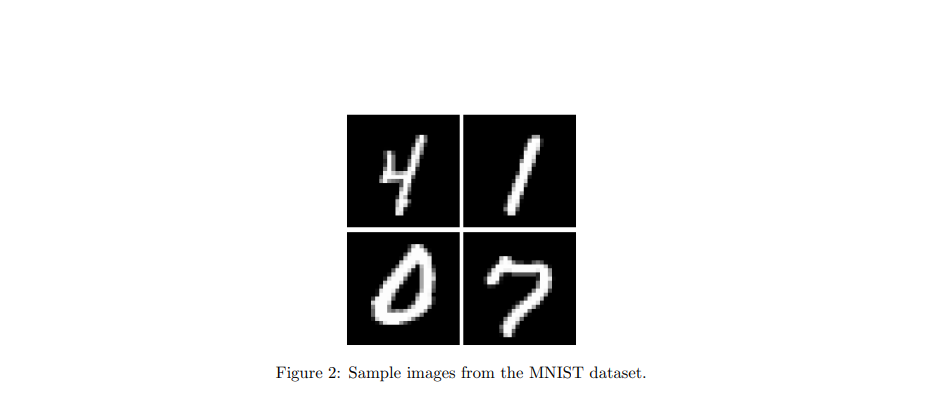
\includegraphics[width=0.8\textwidth]{msit.png}
    \caption{Primal Formulation of SVM}
    \label{fig:primal}
\end{figure}
The classic MNIST dataset (Figure 2) consists of 28x28 pixel (784 features) grayscale images of handwritten
digits 0-9 (10 classes).
In this problem, you will implement a neural network to classify the MNIST dataset using raw pixels as
features. Specifically, you will implement a type of architecture called a Multi-Layered Perceptron (MLP),
which consists of several Dense layers (i.e. “Perceptrons”) connected sequentially, with nonlinear activation
functions after each layer. You will then train this network using the Categorical Cross-Entropy loss function.

Getting Started Download the hw3q6.zip file, which contains starter code for this question, as well as
the MNIST train split (mnist.npz) and the MNIST test split with its labels removed (mnist test.npz).
For this lab, you will need to install Python and Numpy. While our autograder will use Python 3.6.9, you
should be able to use any recent version of Python 3 and Numpy, though you should avoid the newest Python
features such as dataclasses and the walrus operator. We also recommend you install tqdm (progress bar)
and Pandas (tabular data), which will be available on the autograder as well.


\subsection*{6.1 Gradient Derivation [8 points]}
We will begin by deriving the gradients we will need to implement backpropagation. You will derive backward passes for two types of layers: the Exponential Linear Unit (ELU) activation, and a Dense (Fully Connected) layer, then use these derivations to implement the backpropagation algorithm for your neural network.

\subsubsection*{Backpropagation}
Let our feed-forward (also referred to as “sequential”) neural network be described by a series of functions $f_1, \dots, f_n$ with input $x_0$, output $x_n$, loss $L = L(x_n, y^*)$ where $y^*$ is the true label, and the feed-forward relationship:
\[
x_k = f_k(w_k, x_{k-1}).
\]
In our model, these functions $f_1, f_2, \dots, f_n$ will represent our Dense layers and activation functions, and are referred to as modules in our code.

In order to perform gradient descent, we need to compute the gradient for each parameter $\frac{\partial L}{\partial w_k}$, which we can express recursively using the chain rule as:
\[
\frac{\partial L}{\partial w_k} = \frac{\partial L}{\partial x_k} \cdot \frac{\partial x_k}{\partial w_k},
\]
\[
\frac{\partial L}{\partial x_{k-1}} = \frac{\partial L}{\partial x_k} \cdot \frac{\partial x_k}{\partial x_{k-1}}.
\]

where $\frac{\partial L}{\partial x_k}$ are the gradients flowing to the previous layer, and $\frac{\partial x_k}{\partial x_{k-1}}$, $\frac{\partial x_k}{\partial w_k}$ are the Jacobians of layer $f_k$ with respect to $x_{k-1}$ and $w_k$, respectively. Note that since $\frac{\partial L}{\partial x_k}$ is the gradient of a scalar $L$ with respect to a column vector $x_k$, this gradient is a row vector. And $\frac{\partial x_k}{\partial w_k}$ is the gradient of a vector with respect to a vector, which is a matrix.

\subsection*{Softmax Cross Entropy}
This layer combines the Softmax function together with the Cross Entropy Function. The softmax function for the output layer $x_n = \begin{bmatrix} x^{(1)}_n & \dots & x^{(D)}_n \end{bmatrix}$ is described by:
\[
x^{(i)}_n = \frac{\exp(x^{(i)}_{n-1})}{\sum_{j=1}^D \exp(x^{(j)}_{n-1})},
\]
for input $x_{n-1}$, and the Cross Entropy loss function is given by:
\[
L(x_n, y^*) = -\sum_{i=1}^D y^{*(i)} \log x^{(i)}_n,
\]
where $x_n$ are the output weights and $y^*$ are the true labels. Backward propagation through the Softmax Cross Entropy layer can be found by computing the first-order derivatives:
\[
\frac{\partial L}{\partial x^{(i)}_{n-1}} = \frac{\partial}{\partial x^{(i)}_{n-1}} \left( -\sum_{i=1}^D y^{*(i)} \log \frac{\exp(x^{(i)}_{n-1})}{\sum_{j=1}^D \exp(x^{(j)}_{n-1})} \right)
\]
\[
= \frac{\partial}{\partial x^{(i)}_{n-1}} \left( -\sum_{i=1}^D y^{*(i)} x^{(i)}_{n-1} + \sum_{i=1}^D y^{*(i)} \log \sum_{j=1}^D \exp(x^{(j)}_{n-1}) \right)
\]
\[
= \frac{\partial}{\partial x^{(i)}_{n-1}} \left( -\sum_{i=1}^D y^{*(i)} x^{(i)}_{n-1} + \log \sum_{j=1}^D \exp(x^{(j)}_{n-1}) \right) \quad \text{(only one } y^{*(i)} \text{ is 1)}
\]
\[
= -y^{*(i)} + \frac{\exp(x^{(i)}_{n-1})}{\sum_{j=1}^D \exp(x^{(j)}_{n-1})}
\]
\[
= -y^{*(i)} + y_i.
\]
The implementation of this layer is provided to you in \texttt{npnn/layers.py}.


\subsection*{Exponential Linear Unit (ELU)}
The Exponential Linear Unit is a variant of the Rectified Linear Unit (ReLU) activation function that eliminates the zero gradient problem when the input is less than 0. Using ELU as an activation function tends to produce faster convergence with more accurate results than using ReLU. Unlike other activation functions, ELU has an extra $\alpha$ constant, which should be a positive number (a typical choice of $\alpha$ is 1 or 0.9).

The expression of an ELU unit is as follows:
\[
\text{ELU}(x) = 
\begin{cases} 
x & \text{if } x > 0, \\
\alpha(e^x - 1) & \text{otherwise}.
\end{cases}
\]

\subsection*{Dense Layer}
A Dense layer is fully connected with the input features. For a weight matrix $W$ and bias $b$, the output is:
\[
f(x) = Wx + b.
\]
\begin{enumerate}
    \item 
    Find the Jacobian $\frac{\partial x_k}{\partial x_{k-1}}$ for the exponential linear unit, $x_k = \text{ELU}(x_{k-1})$.
    \item
    Find the Jacobian $\frac{\partial x_k}{\partial x_{k-1}}$ for the Dense layer, $x_k = Wx_{k-1} + b$.
    \item 

    Find the Jacobian $\frac{\partial x_k}{\partial b}$ for the Dense layer, $x_k = Wx_{k-1} + b$.
    \item Since $W$ is two-dimensional, the Jacobian $\frac{\partial x_k}{\partial W}$ can only be expressed by matrix-vector multiplications if we flatten it to a vector. Instead, to preserve its dimension, find the gradient $\frac{\partial x_k[a]}{\partial W[b,c]}$ for indices $a$, $b$, $c$ (so that we can write $\frac{\partial x_k}{\partial W}$ as a 3-dimensional tensor). Here, $a$ is an index of $x_k$, $b$ indexes a row of $W$, and $c$ indexes a column of $W$.
\end{enumerate}

\subsection*{6.2 Module Implementation [11 points]}
Implement the ELU and Dense modules based on your answers in the previous part. The correctness of your implementation for parts 6.2 and 6.3 along with your prediction accuracy for part 6.4a will be checked in unit tests, where we will compare your implementation against our implementation.

\textbf{Note:} Do not use any Python libraries other than the ones provided in \texttt{requirements.txt}; otherwise, the autograder will not be able to run your code. In particular, you may not utilize any libraries performing automatic differentiation such as PyTorch, TensorFlow, and JAX in your submitted code, though you may use these libraries to test your implementation if you wish.

\begin{enumerate}
    \item 
    Complete the initialization \texttt{\_\_init\_\_} of the dense layer in \texttt{npnn/modules.py}. You should initialize the bias $b$ to all zeros; $W$ should be initialized using the Glorot Uniform initialization. In the Glorot Uniform initialization, each element is drawn from a uniform distribution $\text{Unif}(-u, u)$, where $u = \sqrt{\frac{6}{\text{dim\_in} + \text{dim\_out}}}$.
    \item 
    In \texttt{npnn/modules.py}, implement forward passes for the ELU and Dense modules.
    \item In \texttt{npnn/modules.py}, implement backward passes for the ELU and Dense modules based on your answer in Problem 6.1.
\end{enumerate}

\subsection*{6.3 Model Training Loop [8 points]}
\begin{enumerate}
    \item 
    In \texttt{npnn/optimizer.py}, implement the \texttt{SGD.apply\_gradients} method.
    \item
    In \texttt{npnn/model.py}, implement forward and backward passes for the model in the \texttt{Sequential.forward} and \texttt{Sequential.backward} methods.
    \item
    In \texttt{npnn/model.py}, implement the training loop in \texttt{Sequential.train}, and the testing method in \texttt{Sequential.test}. To help you organize your implementation, we have provided the signature of categorical cross-entropy and categorical accuracy functions for you to use.
\end{enumerate}


\subsection*{6.4 Training and Evaluation [8 points]}
In order to train your neural network, we have loaded the MNIST dataset included with the starter code (\texttt{mnist.npz}). We have randomly split the dataset into a training dataset with 50,000 elements and a validation dataset with 10,000 elements. Note, we are splitting the MNIST dataset into train and validation and leaving the test set explicitly for testing the model's predictions after completing training. Next, create a neural network with 3 Dense layers with 256, 64, and 10 units, respectively. The first two Dense layers should be followed by an ELU activation with $\alpha = 0.9$, and the last Dense layer should be followed by the \texttt{SoftmaxCrossEntropy} module. See Figure 3 for an illustration of the neural network structure.

When correctly vectorized, your implementation should take fewer than 10 seconds to perform a single epoch during training; see the module docstring for more expected runtime details. While you will not be graded on runtime, excessive runtime may indicate the presence of errors in your code, and it may impact your ability to debug your code and complete experiments in a timely manner.

\textbf{Note:} At this point, you should have implemented all functions or methods annotated with \texttt{\# TODO} or \texttt{raise NotImplementedError()} except for the extra credit implementation of the Adam optimizer.

\begin{figure}[h]
    \centering
    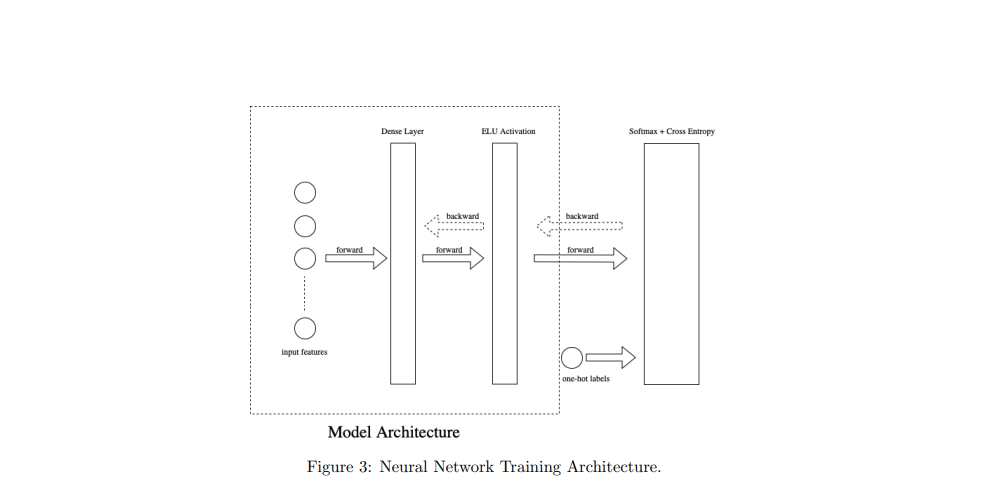
\includegraphics[width=0.8\textwidth]{model.png}
    \caption{Primal Formulation of SVM}
    \label{fig:primal}
\end{figure}


\subsection*{6.4 Training and Evaluation [8 points]}
\begin{enumerate}
    \item \textbf{[2 points]} Train this network for 20 epochs with a learning rate of 0.1 and a batch size of 32, evaluating the network on your validation split after each epoch. Then, plot the train and validation accuracy after each epoch during training.
    
    You should submit two plots along with your answer: one showing a training loss curve and a validation loss curve with respect to the training epochs, and one showing a training accuracy curve and a validation accuracy curve with respect to the training epochs. Make sure to label both curves!

    \item \textbf{[3 points]} Test your trained network on the test dataset (\texttt{mnist\_test.npz}), and submit your predictions to Gradescope. You will receive credit if your test accuracy is greater than 97\%. \textbf{Note:} The \texttt{mnist\_test.npz} dataset does not include the true labels. You can use your validation accuracy to estimate your test accuracy in advance (as long as you perform your train-val split in an unbiased manner).

    \item \textbf{[3 points]} Repeat the training procedure using learning rates of $[0.05, 0.1, 0.2, 0.5, 1.0]$, and plot the lowest validation loss obtained for each learning rate. What is the effect of changing the learning rate? Your plot should be a line graph with the learning rate on the $x$-axis and the best validation loss on the $y$-axis. Since there is a large difference in magnitude for the learning rate, you should use the log-learning rate in your graph, and set the labels manually:
    \begin{verbatim}
    fig, ax = plt.subplots()
    # ... draw plot here ...
    ax.set_xticks([0.05, 0.1, 0.2, 0.5, 1.0])
    ax.set_xticklabels([0.05, 0.1, 0.2, 0.5, 1.0])
    \end{verbatim}
\end{enumerate}
\subsection*{6.5 Bonus: Adam [+5 points]}
The Adam (Adaptive Moment) optimizer is a popular SGD variant (third most popular after SGD and Momentum by citations, according to this paper) that adds “momentum” to the gradients and tries to normalize the gradients by their current magnitude. Adam defines two values for each parameter, $m$ and $v$, which are initialized by zero and updated by the relationship:
\[
m_{t+1} = \beta_1 m_t + (1 - \beta_1) g_t,
\]
\[
v_{t+1} = \beta_2 v_t + (1 - \beta_2) g_t^2,
\]
where $g_t$ is the gradient at time step $t$. Then, the final parameter update is defined by:
\[
\theta_{t+1} = \theta_t - \frac{\eta}{\sqrt{\hat{v}} + \epsilon} \hat{m},
\]
where $\hat{m} = \frac{m_t}{1 - \beta_1}$ and $\hat{v} = \frac{v_t}{1 - \beta_2}$. These updates are controlled by four hyperparameters: $\beta_1$, the momentum decay constant; $\beta_2$, the second moment decay constant; $\eta$, the learning rate; and $\epsilon$, a small constant added to the denominator.

Implement the Adam optimizer in \texttt{npnn/optimizer.py}, and tune the learning rate, setting the other hyperparameters to $\beta_1 = 0.9$, $\beta_2 = 0.999$, $\epsilon = 10^{-7}$. How does a properly-tuned Adam optimizer compare to SGD? How does the sensitivity of Adam to its learning rate compare to SGD?



\end{document}